
\chapter[Suporte Tecnológico]{Suporte Tecnológico}\label{ch:suporteTecnologico}
  Esse capítulo irá apresentar as principais tecnologias envolvidas no desenvolvimento do sistema.
  Desse modo, este  capítulo está dividido nas seções: Aquisição de dados com sensores(\ref{sec:Aquisição de dados com sensores}),
Processamento de sinais(\ref{sec:Processamento de sinais}), Interface humano/computador(\ref{sec:Interface humano/computador}) e
Restrição - Tempo real(\ref{sec:restrição}).

\section{Aquisição de dados com Sensores}
\label{sec:Aquisição de dados com sensores}

  Sensor pode ser entendido como dispositivo eletrônico que é sensível a determinada
condição do ambiente, desde luminosidade, temperatura até a aceleração própria.
Para nosso sistema,  o kinect.

  O kinect é um sensor de movimentos, desenvolvido inicialmente para as plataformas
de jogos eletrônicos da microsoft. Ele possui uma camara RGB(\textit{Red, Green, Blue}),
um sensor de profundidade, um microfone embutido, e a versão mais recente, chamado de kinect 2.0,
consegue detectar 25 articulações esqueletais por pessoa.

\begin{figure}[!h]
\centering
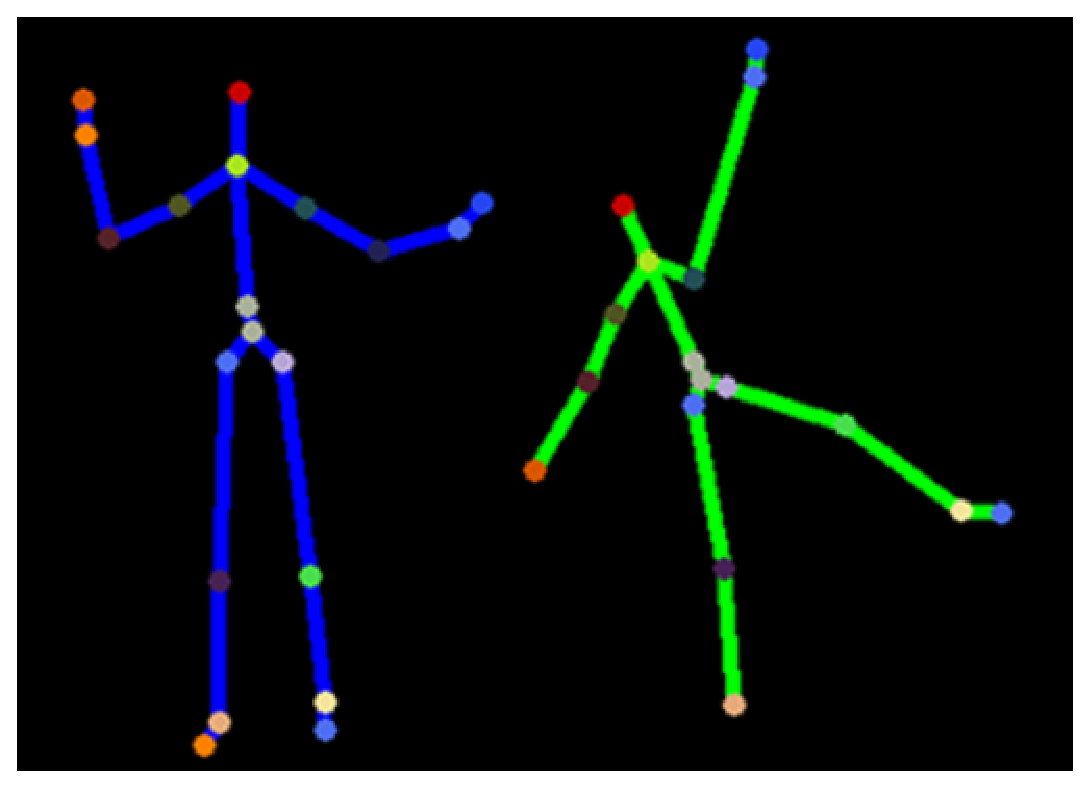
\includegraphics [keepaspectratio=true,scale=0.60]{figuras/esqueletoKinect.eps}
\caption{Esqueleto Kinect}
\cite{microsoftResearch}
\label{esqueletokinect}
\end{figure}

  O windows SDK para Kinect, fornece ferramentas e APIs necessários para desenvolver
aplicações Kinect nas linguagens  C++, C\#, Visual Basic, ou outra linguagem .NET. Hoje em sua versão 2.0. Entre seus recursos estão o acesso completo ao Kinect: vídeo,
profundidade, áudio, motor e funções de alto nível e também  criar aplicativos
para o sistema operacional da microsoft e seu console para jogos.

  Por custos e facilidade de se encontrar, neste sistema utilizaremos a primeira versão do kinect, que possui todas as funcionalidades já citadas, perdendo apenas
em performance.

\section{Processamento de sinais}
\label{sec:Processamento de sinais}
  Os dados obtidos através do sensor serão tratados dentro do Unity 3d, através de suas bibliotecas e com o auxílio da
 linguagem C\#.

\section{Interface humano/computador}
\label{sec:Interface humano/computador}
  O foco principal do sistema é auxiliar pacientes que apresentam deficiência
motoras e ou físicas, para tal é necessário entender os aspectos e
ter conhecimento do padrão dos movimentos.
Optou-se por uma interface com usuário semelhante à jogos, à fim de facilitar a visualização dos movimentos através de avatares customizados e tornar o exercício menos tedioso e mais lúdico.


Para isso o sistema necessita
uma forma de comunicação amigável com o paciente, em conformidade com isto,
temos o motor gráfico para jogos Unity 3D.

  Unity 3d é um motor gráfico, criado para jogos em três e duas dimensões, além de ser
multiplataforma. Com ênfase na portabilidade ele tem como alvo o maior número
de apis gráficas possíveis, desde o sistema operacional da microsoft, o windows,
ao android.  Tem suporte para programação em C\# e JavaScript. O unity 3d também
 possui uma licença pessoal, livre de custos.

  Pela sua capacidade multiplataforma e sua grande comunidade ativa, o unity 3D
é usado neste trabalho para o desenvolvimento do sistema.

%\section{Integração}
%\label{sec:Integração}
%
%  Como já foi especificado, o sistema se dividirá em três módulos, a leitura dos sensores (C\#) o processamento
%de sinais (python), e a interface com o usuário (Unity 3D), para dar vida ao sistema
%precisaremos integrar ambos. A informação que será compartilhada entre esses três
%módulos é dados sobre os ângulos/articulações do movimento. Como uma diretriz inicial,
% temos uma tabela de ângulos entre os sistemas \ref{nomenclaturaUnity3d}.


%\begin{table}[]
%\centering
%\caption{Nomenclatura Unity 3d para as articulações em ordem hierárquica}
%\label{nomenclaturaUnity3d}
%\begin{tabular}{|c|c|c|c|c}
%\cline{1-4}
%\multicolumn{4}{|c|}{\cellcolor[HTML]{9B9B9B}\textbf{Nomenclatura Unity3d para as articulações em ordem hierárquica}}             &  \\ \cline{1-4}
%\cellcolor[HTML]{C0C0C0}Nome & \cellcolor[HTML]{C0C0C0}Tipo & \cellcolor[HTML]{C0C0C0}Grupo & \cellcolor[HTML]{C0C0C0}Equivalente &  \\ \cline{1-4}
%Hips                         & Normal                       & Body                          & Quadril                             &  \\ \cline{1-4}
%Spine                        & Normal                       & Body                          & Espinha                             &  \\ \cline{1-4}
%Spine                        & Normal                       & Body                          & Espinha                             &  \\ \cline{1-4}
%Chest                        & Optional Bone                & Body                          & Peito                               &  \\ \cline{1-4}
%                             &                              &                               &                                     &  \\ \cline{1-4}
%Shoulder                     & Optional Bone                & Left Arm/Right Arm            & Ombro                               &  \\ \cline{1-4}
%Upper Arm                    & Normal                       & Left Arm/Right Arm            & Braço                               &  \\ \cline{1-4}
%Lower Arm                    & Normal                       & Left Arm/Right Arm            & Antebraço                           &  \\ \cline{1-4}
%Hand                         & Normal                       & Left Arm/Right Arm            & Mão                                 &  \\ \cline{1-4}
%                             &                              &                               &                                     &  \\ \cline{1-4}
%Upper leg                    & Normal                       & Left leg/Right leg            & Coxa                                &  \\ \cline{1-4}
%Lower leg                    & Normal                       & Left leg/Right leg            & Canela                              &  \\ \cline{1-4}
%Foot                         & Normal                       & Left leg/Right leg            & Pé                                  &  \\ \cline{1-4}
%Toes                         & Optional Bone                & Left leg/Right leg            & Dedos                                  &  \\ \cline{1-4}
%\end{tabular}
%\end{table}

\subsection{Articulações no Unity 3d}
\label{sec:Articulacoes no Unity 3d}
  Também chamadas de character joint elas são usadas para o chamado efeito
boneco de pano (\textit{ragdoll effects}). A posição inicial de Referência é a
a posição em T (\textit{T pose}). O unity não limita a angulação da articulação,
deixando isso na mão do desenvolvedor, porém eles orientam ângulos máximos
para estabilizar melhor seu avatar 3d.\cite{unity3dManual}

\subsection{Articulações no corpo humano}
\label{sec:Juntas no corpo humano}
 A posição anatômica é uma posição de referência, que dá significado aos termos
 direcionais utilizados na descrição das partes e regiões do corpo. As discussões
 sobre o corpo, o modo como se movimenta, sua postura ou a relação entre uma e
outra área assumem que o corpo como um todo está numa posição específica chamada
 posição anatômica

  A tabela \ref{Juntas no corpo} mostra a articulação, seus movimentos e sua capacidade máxima em
graus de movimentações.

\begin{table}[]
\centering
\caption{Articulações no corpo}
\label{Juntas no corpo}
\begin{tabular}{|c|c|c|}
\hline
\rowcolor[HTML]{C0C0C0}
Articulação                 & Movimento       & Grau de  Movimento \\ \hline
                            & Flexão          & 0-180              \\ \cline{2-3}
                            & Extensão        & 0-45               \\ \cline{2-3}
                            & Adução          & 0-40               \\ \cline{2-3}
                            & Abdução         & 0-180              \\ \cline{2-3}
                            & Rotação medial  & 0-90               \\ \cline{2-3}
\multirow{-6}{*}{Ombro}     & Rotação lateral & 0-90               \\ \hline
                            & Flexão          & 0-145              \\ \cline{2-3}
\multirow{-2}{*}{Cotovelo}  & Extensão        & 145-0              \\ \hline
                            & Pronação        & 0-90               \\ \cline{2-3}
\multirow{-2}{*}{Radiulnar} & Supinação       & 0-90               \\ \hline
                            & Flexão          & 0-90               \\ \cline{2-3}
                            & Extensão        & 0-70               \\ \cline{2-3}
                            & Adução          & 0-45               \\ \cline{2-3}
\multirow{-4}{*}{Punho}     & Abdução         & 0-20               \\ \hline
\end{tabular}
\end{table}

\section{Restrição - Tempo real}
\label{sec:restrição}
  Todo o processo desde a aquisição do movimento ao processamento do sinal e a
resposta para o usuário pode ser feito sequencialmente, porém ele deve dar o
retorno em tempo real para que o usuário possa corrijir a movimentação e se
aproxime da correta execução do movimento. Para isso, temos que levar em conta
a frequência de aquisição do sensor usado, o tempo do processamento de sinal e
a frequência de atualização do monitor.

  O sensor kinect \cite{microsoftResearch}, tem uma frequência de
aquisição de quadros de 30Hz, junto a um monitor com taxa de atualização de imagem
para o usuário a 30Hz, assim a aproximadamente 33 milisegundos o
sistema recebe um input do sensor e tem que em seguida apresentar um output. Isso
 restringe o processamento do sinal a 33 milissegundo de um input a outro, e
também no tempo de atualização da imagem exibida para que não haja perda na
fluidez e nem atraso na correção.
